\documentclass[pscyr, nonums]{hedlab}
\usepackage[russian]{babel}
\usepackage[utf8]{inputenc}
\usepackage{graphicx}
\usepackage{listings}

\graphicspath{{images/}}

\lstset{
    basicstyle=\scriptsize,
    inputencoding=utf8,
    extendedchars=\true,
    language=[Sharp]C,
    numbers=left,
    numberstyle=\scriptsize,
    breakatwhitespace=\false,
    breaklines=True,
    tabsize=2,
    keepspaces=true,
}

\labnum{4}
\labname{Создание многостраничного приложения на Silverlight}
\student{Голубев А. В.}
\date{}

\begin{document}
    \makeheader
    \emph{Цель работы:} получение общих сведений о технологии Silverlight, получение практических навыков создания web-приложений, использующий Silverlight.

    \emph{Задачи:}
    \begin{enumerate}\itemsep-5pt
        \item Создать web-приложение на ASP.NET
        \item Создать многостраничную Silverlight-форму
        \item Добавить созданную форму на разные страницы web-приложения на ASP.NET 
        \item Добавить на Silverlight-форму элементы управления и обработчики событий.
        \item Соотнести разные страницы Silverlight-формы с разными страницами web-приложения на ASP.NET
    \end{enumerate}

    \emph{Скриншоты:}
    \begin{figure}[ht]
        \center
        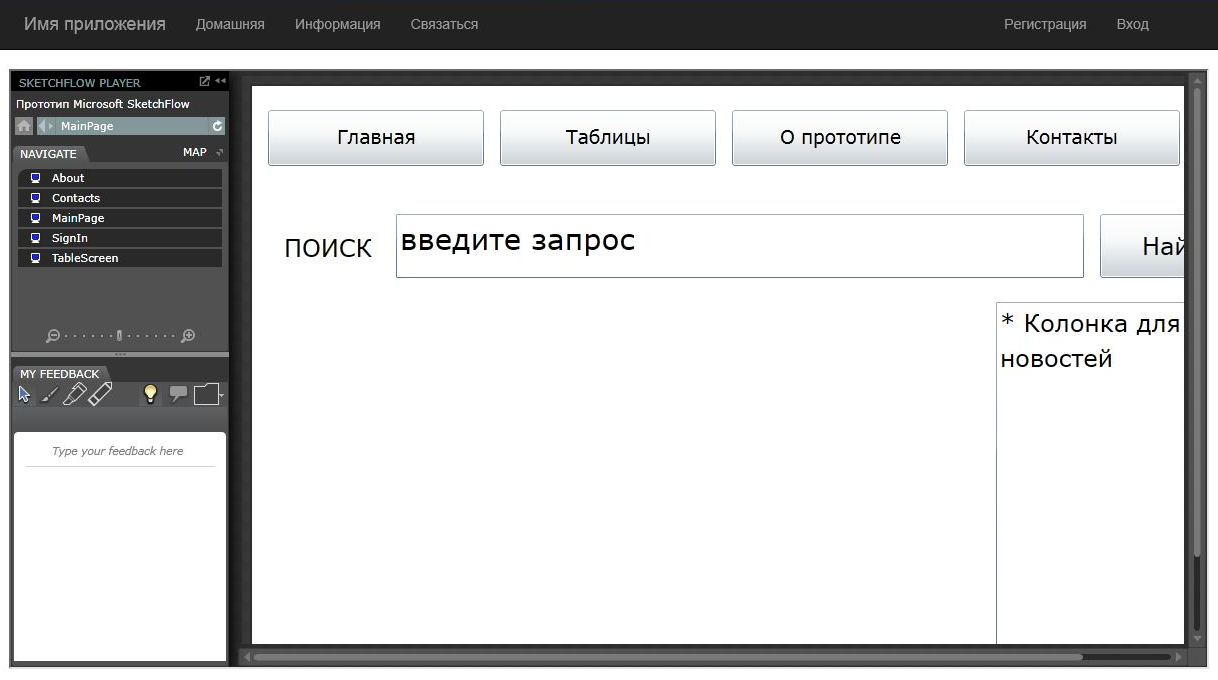
\includegraphics[width=1\textwidth]{Lab04_01}
        \caption{Главная страница с Silverlight-формой}
    \end{figure}

    \pagebreak

    \begin{figure}[ht]
        \center
        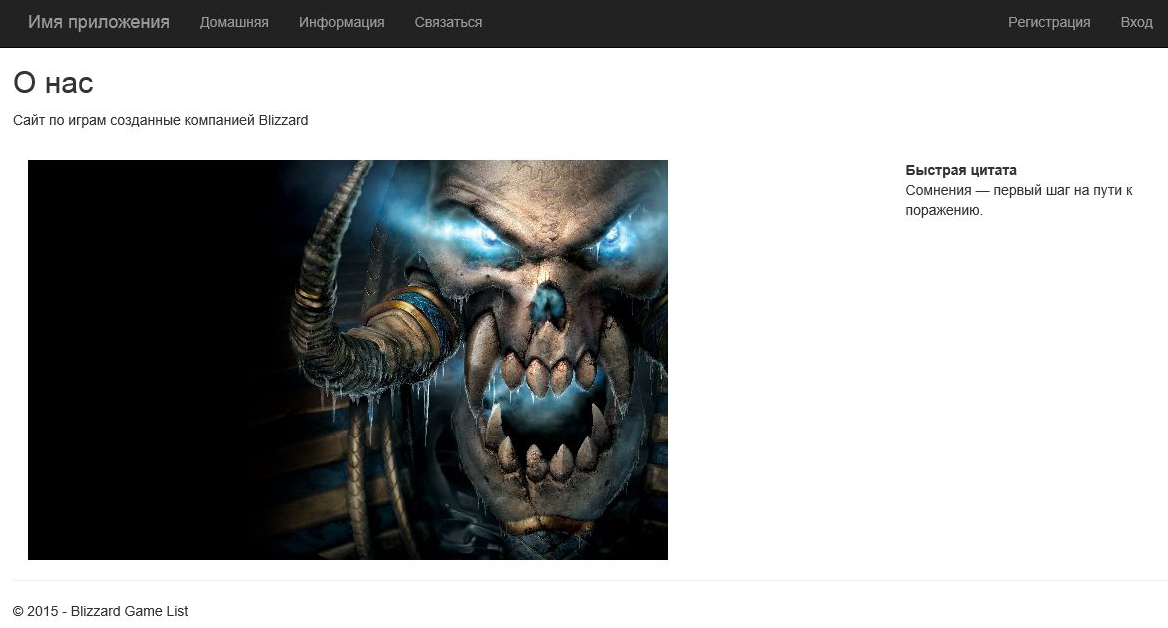
\includegraphics[width=1\textwidth]{Lab04_02}
        \caption{О сайте}
    \end{figure}
    \begin{figure}[ht]
        \center
        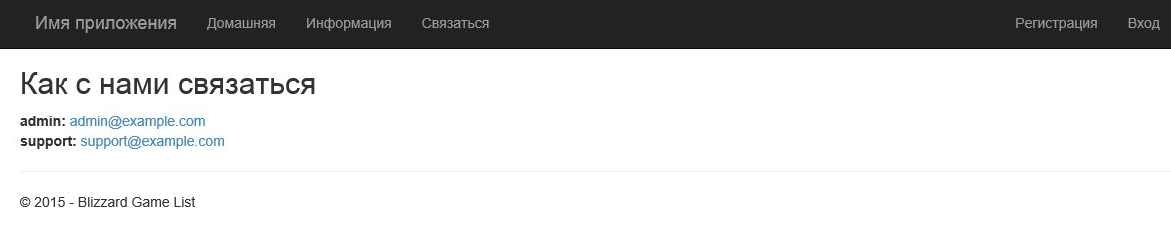
\includegraphics[width=1\textwidth]{Lab04_03}
        \caption{Контактная информация}
    \end{figure}

    \pagebreak

    \begin{figure}[ht]
        \center
        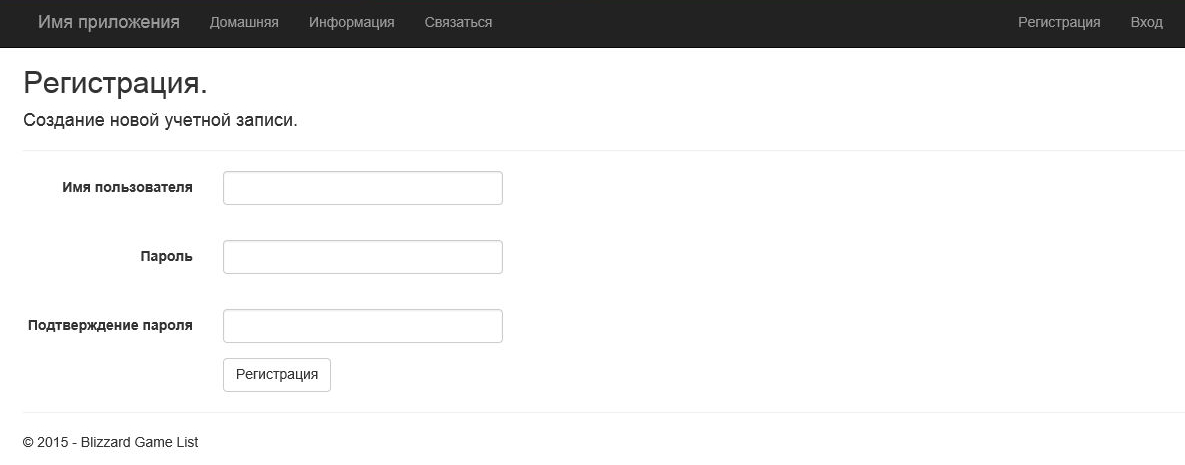
\includegraphics[width=1\textwidth]{Lab04_04}
        \caption{Регистрация}
    \end{figure}
    \begin{figure}[ht]
        \center
        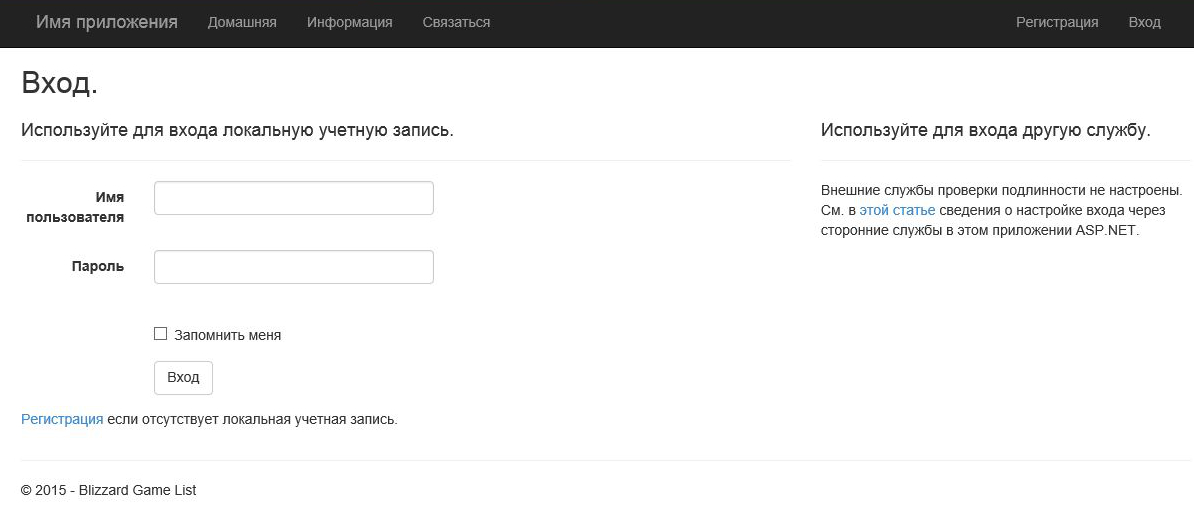
\includegraphics[width=1\textwidth]{Lab04_05}
        \caption{Вход}
    \end{figure}

    \pagebreak

    \emph{Исходный код:}
    \begin{center}
        \textbf{Страница About}
    \end{center}
    \lstinputlisting{./source/About.aspx.cs}

    \begin{center}
        \textbf{Страница Login}
    \end{center}
    \lstinputlisting{./source/Login.aspx.cs}

    \begin{center}
        \textbf{Страница Register}
    \end{center}
    \lstinputlisting{./source/Register.aspx.cs}

    \begin{center}
        \textbf{Вспомогательный код для регистрации}
    \end{center}
    \lstinputlisting{./source/Manage.aspx.cs}
    \lstinputlisting{./source/OpenAuthProviders.ascx.cs}
    \lstinputlisting{./source/RegisterExternalLogin.aspx.cs}
\end{document}
